\documentclass[10pt, twocolumn]{article}
\usepackage[margin=0.70in]{geometry}
\usepackage{graphicx}
\usepackage{amsmath}
\usepackage{booktabs}
\usepackage{hyperref}
\usepackage[numbers]{natbib}
\usepackage{titling}
\usepackage{caption}
\usepackage{pdfpages}
\captionsetup{font=small, skip=4pt}
\graphicspath{{figures/}}
        
\title{\vspace{-1.5cm}Reproducing and Improving TypiClust\vspace{-0.5cm}}
\author{Lucas Lobo - k23075501}
\date{}

\begin{document}
\maketitle
\vspace{-0.8cm}

\section{Introduction}
Deep learning requires large labelled datasets, yet annotation is costly. Active Learning (AL) mitigates this by iteratively selecting informative unlabelled examples, but traditional uncertainty-based methods rely on a trained model, creating a cold start problem. Hacohen et al.~\cite{hacohen2022active} identified that the optimal AL strategy depends on budget size: typical examples should be queried first, with 
  uncertainty-based methods taking over once sufficient labels exist. They proposed TypiClust, which selects typical points from K-Means clusters in a self-supervised representation space. However, typicality alone can produce redundant selections. We reproduce TypiClust on CIFAR-10 and propose a hybrid modification incorporating diversity-aware selection.

\section{Methodology}

\subsection{TypiClust Pipeline}

Our implementation follows the TPC$_{RP}$ variant for initial pool selection ($L_0 = \emptyset$). Following the paper, we train a SimCLR~\cite{chen2020simple} encoder (ResNet-18, 200 epochs) from scratch on CIFAR-10, producing 512-d embeddings. We simplify the training setup: Adam optimiser (vs.\ LARS), batch size 256 (vs.\ 4096), and no cosine LR schedule --- reducing training to $\sim$2 hours on a single GPU versus the paper's TPU-scale setup. This narrows the TPC$_{RP}$ accuracy gap by $\sim$4\% vs.\ the paper (44.4\% vs.\ $\sim$48\%) while the random baseline remains comparable (36.9\% vs.\ $\sim$38\%), confirming that relative method ordering is preserved. K-Means with $K = B$ partitions embeddings into $B$ clusters, and from each the point with the highest typicality is selected:
\begin{equation}
    \text{Typicality}(x) = \left(\frac{1}{k}\sum_{x_i \in \text{KNN}(x)} \|x - x_i\|_2\right)^{-1}
\end{equation}
where $k = 20$ neighbours. Higher values indicate points more central to the data distribution. Selection quality is evaluated via a linear probe (logistic regression on frozen embeddings), isolating the effect of sample selection from representation quality.

\subsection{Proposed Modification}

Even though TypiClust demonstrates strong performance in low-budget regimes, selecting points based purely on typicality can still choose examples that are spatially close in the embedding space, underrepresenting regions of the data distribution. This motivates incorporating spatial diversity, a principle exploited by CoreSet~\cite{sener2018active}. We propose the following modifications:

\textbf{Hybrid Score Formula.} We replace the pure typicality criterion with a hybrid score:
\begin{equation}
    \text{score} = \alpha \cdot \hat{t} + (1 - \alpha) \cdot \hat{d}
\end{equation}
where $\hat{t}$ is the normalised typicality and $\hat{d}$ is the normalised minimum distance to already-selected points, both scaled to $[0,1]$ within each cluster. This balances representativeness with spatial diversity, reducing redundancy among selected examples. Selection proceeds sequentially: the most typical point overall is chosen first, and each subsequent point is scored considering distance from already-selected points.

\textbf{Dimensionality Reduction.} High-dimensional embeddings (512-d) can suffer from the curse of dimensionality~\cite{aggarwal2001surprising}, where distance metrics become less meaningful. We apply PCA and UMAP~\cite{mcinnes2018umap} to reduce dimensionality before clustering. UMAP is chosen over alternatives such as t-SNE because it preserves both local and global structure and supports transforming unseen test data, which is necessary for consistent evaluation. However, UMAP introduces additional hyperparameters ($n\_components$) and stochasticity.

\textbf{Alpha Tuning.} The parameter $\alpha$ controls the trade-off between typicality and diversity: $\alpha = 1$ recovers the original TypiClust selection, while $\alpha = 0$ selects purely for maximum distance. We sweep $\alpha$ across $[0, 1]$ to find the optimal balance.

\section{Results}

\subsection{Paper Results}

Table~\ref{tab:paper} summarises key results from~\cite{hacohen2022active} on CIFAR-10 ($B=10$). Both TypiClust variants outperform all baselines in the low-budget regime. In the semi-supervised setting with FlexMatch, TypiClust reaches 93.2\% accuracy (+39.4\% over random). As budget grows, uncertainty methods eventually surpass TypiClust, confirming the phase transition.

\begin{table}[h!]
    \centering\small
    \begin{tabular}{lccc}
        \toprule
        Strategy & Supervised & SS Embed. & Semi-sup. \\
        \midrule
        Random     & $\sim$18\% & $\sim$38\% & 53.8\% \\
        Uncertainty & $\sim$15\% & $\sim$35\% & -- \\
        TPC$_{RP}$ & $\sim$\textbf{28\%} & $\sim$\textbf{48\%} & \textbf{93.2\%} \\
        \bottomrule
    \end{tabular}
    \caption{Paper results on CIFAR-10 ($B=10$, first AL round). Supervised and SS Embedding values estimated from~\cite{hacohen2022active} Figs.\ 4--5.}
    \label{tab:paper}
\end{table}

\subsection{Our Results}

We reproduce TPC$_{RP}$ on CIFAR-10 with $B = 10$. To address the single-run limitation, we evaluate each method across 10 K-Means random seeds and report mean accuracy $\pm$ standard deviation. A random baseline is established over 30 seeds, yielding $36.92\% \pm 6.75\%$.

The baseline TypiClust reproduction achieves $44.42\% \pm 0.42\%$, covering 7 out of 10 classes on average. While this confirms that typicality-based selection outperforms random sampling, the limited class coverage motivates our modifications. The alpha sweep (Figure~\ref{fig:alpha_sweep}) shows that introducing hybrid selection ($\alpha = 0.4$) raises accuracy to $53.34\%$ with full class coverage (10/10), demonstrating that diversity substantially reduces redundancy. Adding PCA dimensionality reduction ($n = 10$, $\alpha = 0.55$) improves accuracy to $57.75\%$, though class coverage drops to 8, suggesting that PCA's linear projection can merge semantically distinct clusters, a trade-off between tighter clusters and class separation. Figure~\ref{fig:umap_heatmap} reveals that the best result is UMAP ($n = 5$) with hybrid selection ($\alpha = 0.2$): $65.78\% \pm 1.71\%$ covering 9.6 classes on average, an improvement of $+21.36\%$ over baseline (Figure~\ref{fig:summary}). This configuration favours diversity ($\alpha = 0.2$), indicating that in UMAP's compact space, spatial separation becomes the dominant factor. The non-zero variance across seeds reflects UMAP's stochastic nature, though the improvement remains highly significant.

\begin{figure}[t]
    \centering
    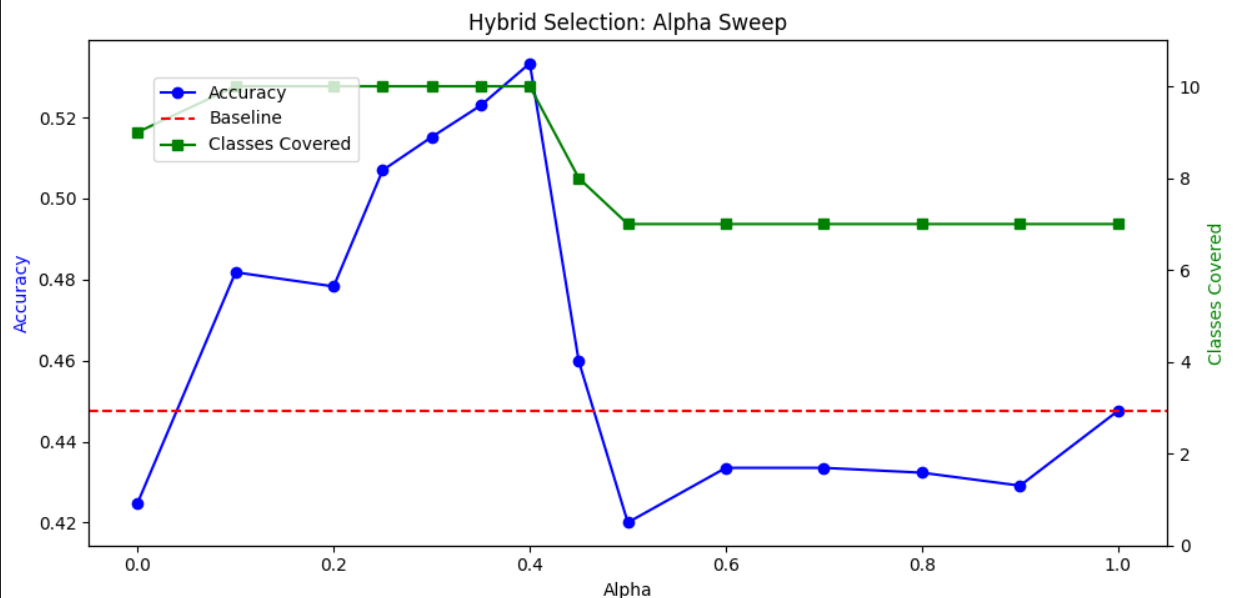
\includegraphics[width=\columnwidth]{alpha_sweep.png}
    \caption{Hybrid selection on CIFAR-10 ($B=10$): accuracy and class coverage vs.\ $\alpha$. Dashed line shows baseline TypiClust.}
    \label{fig:alpha_sweep}
\end{figure}

\begin{figure}[t]
    \centering
    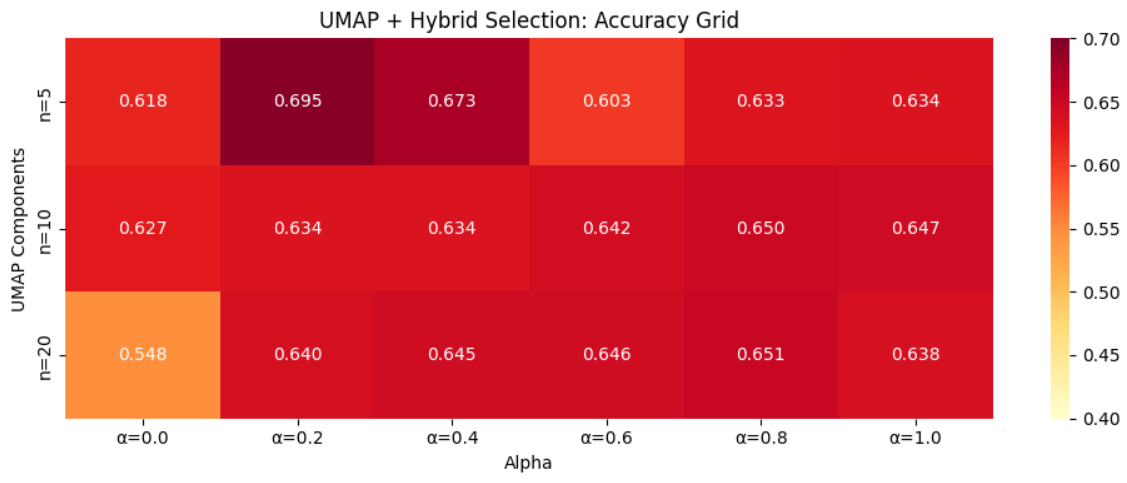
\includegraphics[width=\columnwidth]{umap_heatmap.png}
    \caption{UMAP + hybrid accuracy grid on CIFAR-10 ($B=10$) across UMAP dimensions and $\alpha$.}
    \label{fig:umap_heatmap}
\end{figure}

\begin{figure}[h!]
    \centering
    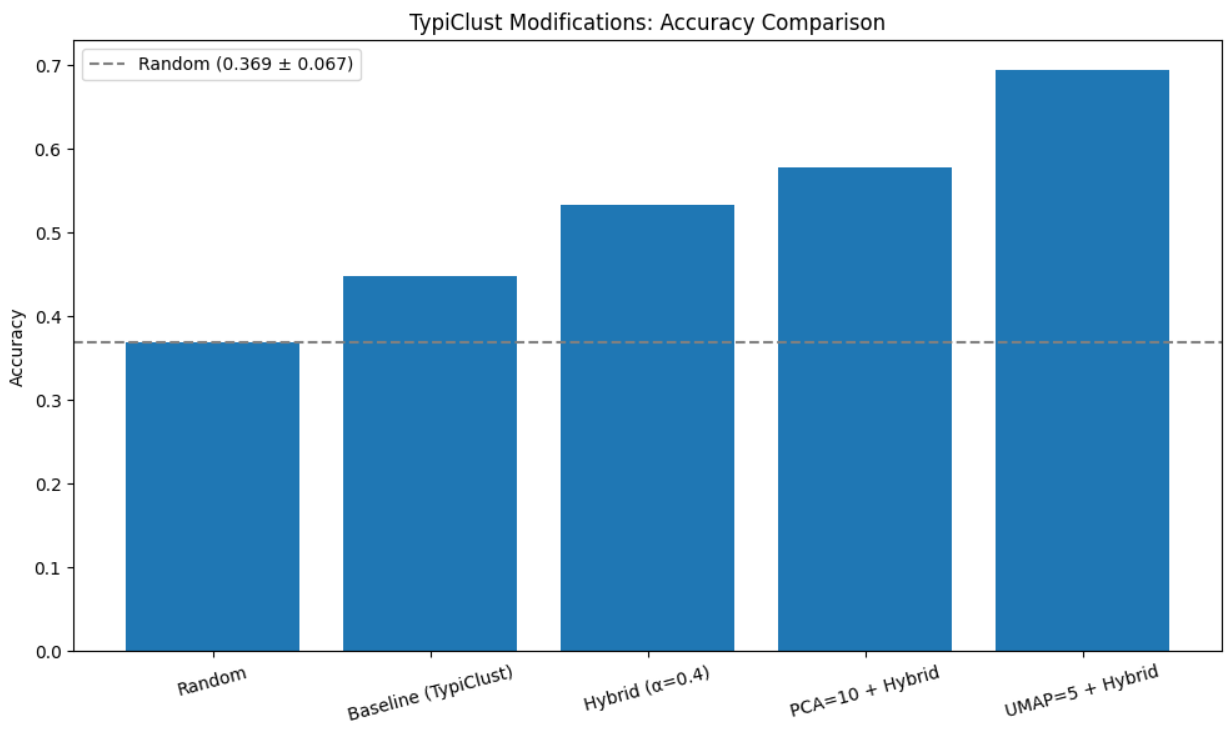
\includegraphics[width=\columnwidth]{summary_bar.png}
    \caption{Accuracy comparison across all selection methods on CIFAR-10 ($B=10$). Error bars show $\pm 1$ std over 10 seeds.}
    \label{fig:summary}
\end{figure}

We also evaluate over-clustering ($K > B$) across multipliers ($2\times$--$10\times$) with both PCA and UMAP preprocessing. Over-clustering consistently degrades performance, validating the paper's $K = B$ design.

\begin{table}[h!]
    \centering
    \begin{tabular}{lcc}
        \toprule
        Method & Accuracy & Classes \\
        \midrule
        Random (30 seeds) & $(36.92 \pm 6.75)\%$ & -- \\
        TypiClust (baseline) & $(44.42 \pm 0.42)\%$ & 7 \\
        Hybrid ($\alpha=0.4$) & $(53.34 \pm 0.00)\%$ & 10 \\
        PCA-10 + Hybrid & $(57.75 \pm 0.00)\%$ & 8 \\
        UMAP-5 + Hybrid & $\mathbf{(65.78 \pm 1.71)\%}$ & 9.6 \\
        \bottomrule
    \end{tabular}
    \caption{Selection strategies on CIFAR-10 ($B=10$), averaged over 10 seeds.}
    \label{tab:results}
\end{table}

\section{Statistical Analysis}

We compare each method (10 seeds) against the random baseline (30 seeds) using two-sample $t$-tests. All achieve significance: baseline ($t = 3.42$, $p = 0.0015$, $d = 1.57$), hybrid ($t = 7.50$, $p < 0.001$, $d = 3.44$), PCA + hybrid ($t = 9.52$, $p < 0.001$, $d = 4.37$), UMAP + hybrid ($t = 13.05$, $p < 0.001$, $d = 5.86$). The progressively increasing Cohen's $d$ values confirm that each modification adds a practically meaningful improvement, not just statistical noise. With Bonferroni correction ($\alpha_{\text{adj}} = 0.0125$), all remain significant. Hybrid and PCA show zero variance due to K-Means stability ($n\_init = 10$); UMAP variance ($\sigma = 1.71\%$) reflects its stochastic initialisation.

\section{Conclusion}

TypiClust's typicality-based selection outperforms random sampling in the low-budget regime, consistent with~\cite{hacohen2022active}. Our hybrid modification improves accuracy from 44.42\% to 65.78\% with UMAP ($+21.36\%$), suggesting the original pipeline underutilises embedding geometry. Over-clustering is detrimental, validating $K = B$.

\textbf{Limitations \& Future Work.} Evaluation is limited to CIFAR-10 ($B=10$) with a linear probe. UMAP adds cost and stochasticity. Future work: multi-round AL, semi-supervised integration, and larger datasets.

\noindent\textbf{Code:} \url{https://github.com/LucasPRLobo/ml-cw2}


\bibliographystyle{plainnat}
{\footnotesize
\begin{thebibliography}{5}
\bibitem[Hacohen et~al.(2022)]{hacohen2022active}
G.~Hacohen, A.~Dekel, and D.~Weinshall.
Active learning on a budget: Opposite strategies suit high and low budgets.
\emph{ICML}, PMLR 162, 2022.
\bibitem[Chen et~al.(2020)]{chen2020simple}
T.~Chen, S.~Kornblith, M.~Norouzi, and G.~Hinton.
A simple framework for contrastive learning of visual representations.
\emph{ICML}, pp.\ 1597--1607, 2020.
\bibitem[McInnes et~al.(2018)]{mcinnes2018umap}
L.~McInnes, J.~Healy, and J.~Melville.
UMAP: Uniform manifold approximation and projection for dimension reduction.
\emph{arXiv:1802.03426}, 2018.
\bibitem[Sener \& Savarese(2018)]{sener2018active}
O.~Sener and S.~Savarese.
Active learning for convolutional neural networks: A core-set approach.
\emph{ICLR}, 2018.
\bibitem[Aggarwal et~al.(2001)]{aggarwal2001surprising}
C.~C. Aggarwal, A.~Hinneburg, and D.~A. Keim.
On the surprising behavior of distance metrics in high dimensional space.
\emph{ICDT}, pp.\ 420--434, 2001.
\end{thebibliography}
}

\clearpage
\onecolumn
\section*{Additional Plots}

\begin{figure}[h!]
    \centering
    \begin{minipage}{0.48\textwidth}
        \centering
        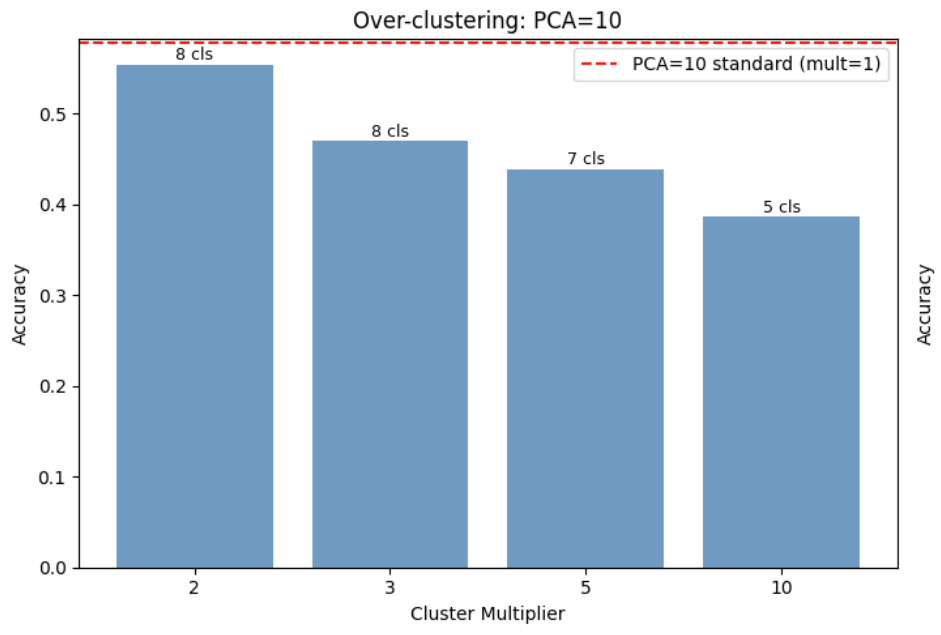
\includegraphics[width=\textwidth]{overclustering_pca.png}
    \end{minipage}
    \hfill
    \begin{minipage}{0.48\textwidth}
        \centering
        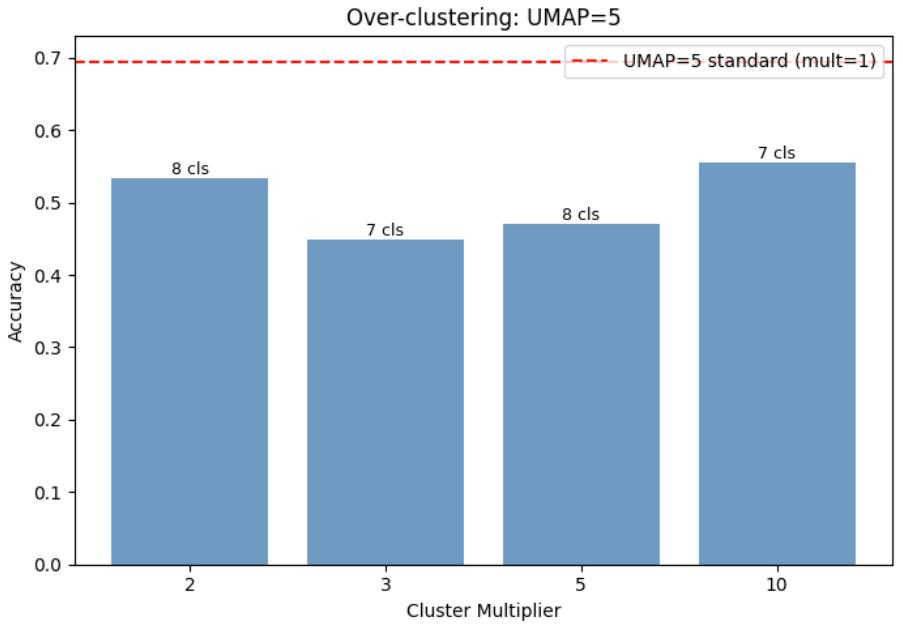
\includegraphics[width=\textwidth]{overclustering_umap.png}
    \end{minipage}
    \caption{Over-clustering ablation for PCA-10 (left, $\alpha=0.55$) and UMAP-5 (right, $\alpha=0.2$). Dashed lines: standard $K=B$ result. Over-clustering consistently degrades performance.}
    \label{fig:overclustering}
\end{figure}

\begin{figure}[h!]
    \centering
    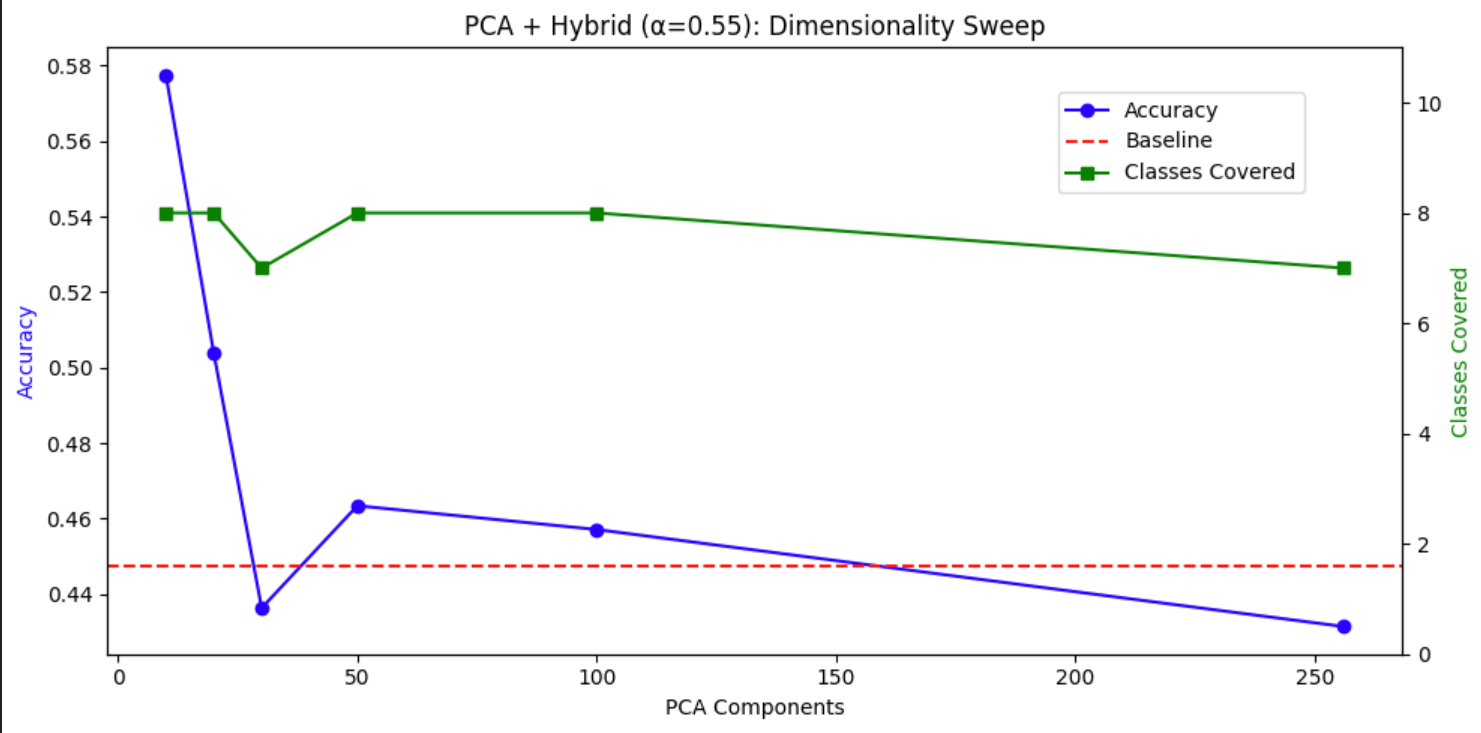
\includegraphics[width=0.65\textwidth]{pca_sweep.png}
    \caption{PCA + hybrid ($\alpha=0.55$): accuracy and class coverage across PCA dimensions.}
    \label{fig:pca_sweep}
\end{figure}

\clearpage

\includepdf[pages=-]{original_algorithm.pdf}

\includepdf[pages=-]{modified_algorithm.pdf}

\includepdf[pages=-]{SimCLR_implementation.pdf}

\end{document}
